\chapter{What the model has been tested on}
\label{app:validation}

\devnote{All results here are for the cloud on the \code{pb-electrons} branch, from seed scans of one system. They
show what the options do to each other; they are not a comparison with experiment or with a reference code.}

\section{Against gromacs-mc}

The field-free cloud is \code{gromacs-mc}'s model.
Started from the same charges and a seeded cloud (\env{GMX\_SFMD\_PB\_SEED}, \file{test/pb\_vs\_mc.sh}), the two codes give
bit-identical clouds, forces and trajectories, with the laser options off.
The force field is the same code in both.

\section{The scans}

Hen egg-white lysozyme (PDB 1AKI, 1960 atoms) in vacuum; 850\,nm, 15\,fs FWHM, peak at 35\,fs, 30\,$\mu$m focus; peak
intensities $10^{15}$, $10^{16}$ and $10^{17}$\,W/cm$^2$; 2\,as; 75\,fs ($10^{16}$, $10^{17}$) or 200--300\,fs
($10^{15}$); 8 seeds per setting, run on the \code{davinci} cluster.
Directions are the heavy-atom displacement directions at the end, compared as the median angle between two settings'
seed-averaged directions, for the fastest 25\,\% of the heavy atoms and for all; the noise is the same comparison
between halves of the seeds, or a seed against the mean of the others.

\begin{figure}[p]
  \centering
  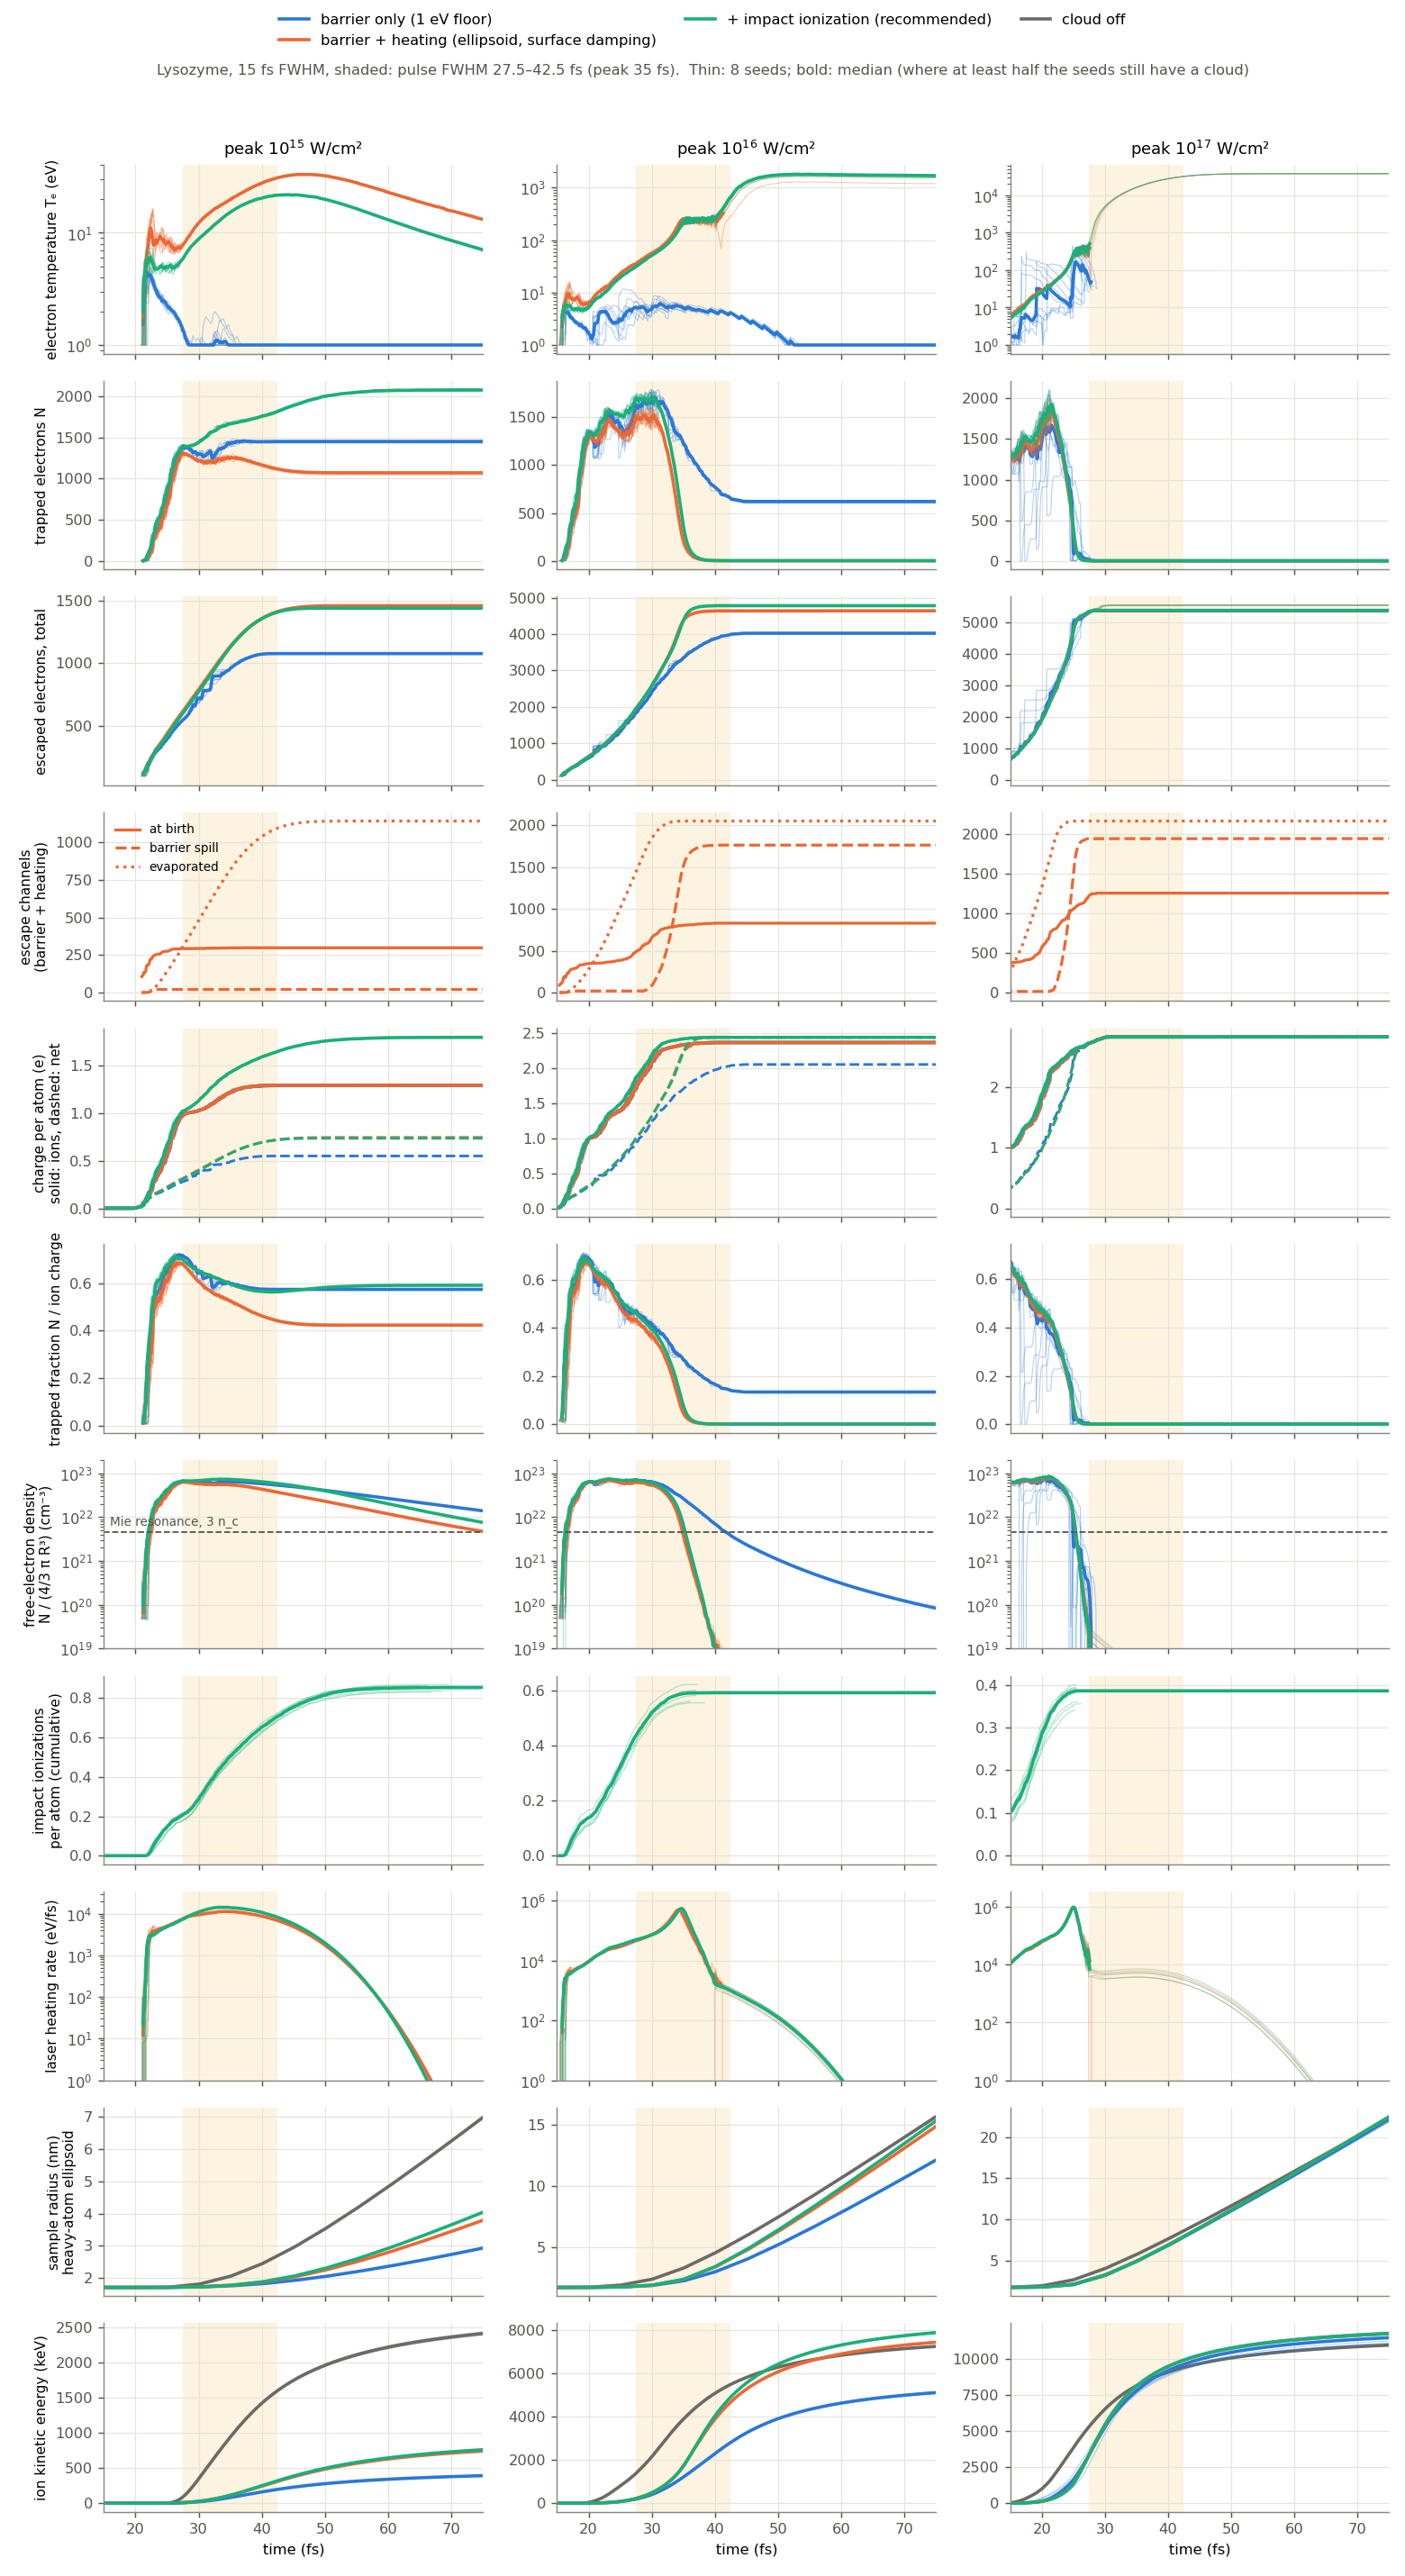
\includegraphics[width=0.92\textwidth]{fig/timeseries.png}
  \caption{The cloud over time, lysozyme, 8 seeds (thin) and their median (bold), for the current model built up step
  by step --- the barrier alone, with heating (ellipsoid, surface damping), and the recommended model with impact
  ionization --- against the cloud off; all with the 1\,eV temperature floor, 75\,fs (scan of 13 November 2026,
  build ref-pb17). With surface damping the heating passes the Mie resonance as a smooth maximum near the pulse peak;
  the earlier scan without it had 15--19\,MeV spikes in about 1 of 8 runs.}
  \label{fig:timeseries}
\end{figure}

\section{What the cloud does}

\begin{table}[H]
\centering\small
\begin{tabularx}{\textwidth}{@{}l X X X@{}}
\toprule
peak [W/cm$^2$] & trapped at the end & ion energy vs cloud off & direction shift vs cloud off (fast 25\,\% / all) \\
\midrule
$10^{15}$ & 59\,\% of the electrons & 0.32 & 8.7$^\circ$ / 13.9$^\circ$ \\
$10^{16}$ & 0 (gone by $\sim$45\,fs) & 1.09 & 3.7$^\circ$ / 5.7$^\circ$ \\
$10^{17}$ & 0 (gone by $\sim$28\,fs) & 1.07 & 3.4$^\circ$ / 5.1$^\circ$ \\
\bottomrule
\end{tabularx}
\caption{The cloud's effect in the recommended model (barrier, heating with the ellipsoid and surface damping, impact
ionization, 1\,eV floor; ref-pb17, 8 seeds, 75\,fs) against the cloud off. The seed spread of the fast ions' directions
(half against half) is 0.6--2.3$^\circ$, so the shifts are systematic. An earlier scan without surface damping, the
ellipsoid and the floor gave 47\,\% trapped, 0.31 and 6.5$^\circ$/8.7$^\circ$ at $10^{15}$, 1.01 and 3.4$^\circ$/4.7$^\circ$
at $10^{16}$.}
\end{table}
At $10^{17}$\,W/cm$^2$ the cloud leaves before the peak, but it holds the sample compact while ADK charges it, which gives
the ions about 7\,\% more energy than without it.

\section{Each option}

\begin{longtable}{@{}p{0.28\textwidth}p{0.66\textwidth}@{}}
\toprule
option & effect on lysozyme \\
\midrule
\endhead
field-free cloud & traps $\sim$98\,\% of the electrons at every intensity: wrong at high intensity \\
barrier, no heating & the cloud cools to the 1\,eV floor; at $10^{15}$ seed-bistable (1196 $\pm$ 436 trapped, ion energy
  701 $\pm$ 541\,keV) \\
heating & reproducible (1139 $\pm$ 9 trapped, 666 $\pm$ 2\,keV at $10^{15}$); at $10^{16}$ the trapped fraction drops from
  13\,\% to 1\,\% \\
collision-rate cap & 1 and no cap agree; 0.1 heats less (1393 trapped at $10^{15}$); 0.5 with the full model: $-16$\,\%
  heating and $-8$\,\% ion energy at $10^{15}$, nothing at $10^{16}$; directions unchanged \\
ellipsoid shape & $+13$\,\% heating, $+6$\,\% ion energy at $10^{15}$; $\sim$1\,\% at $10^{16}$; directions within noise \\
surface damping ($A=1$) & removes the resonance outliers (15--19\,MeV in 1 of 8 runs); seed spread of the ion energy at
  $10^{16}$ $\pm$90 $\to$ $\pm$28\,keV; ion energy $+2.5$\,\% ($10^{15}$), $+7$\,\% ($10^{16}$), $+1.6$\,\% ($10^{17}$);
  $A$ = 0.5 / 1 / 2: 7806 / 7912 / 7986\,keV at $10^{16}$ \\
barrier mode 2 & same charges, energies (within 2\,\%) and directions as mode 1; clamped energy in 3 of 24 runs \\
impact ionization & ion charge 1.29 $\to$ 1.72 per atom at $10^{15}$, +2.5\,\% at $10^{16}$; net charge and directions
  unchanged, ion energy $+6$\,\% ($10^{15}$) \\
recombination 2 & gives the charge back after the pulse (1.72 $\to$ 1.35), explosion unchanged \\
recombination 1 & capture--ADK pump: ADK events 1868 $\to$ 17\,284, ion energy $+22$\,\% \\
temperature floor 1\,eV & acts $\sim$0.02\,fs per run; ion energy 927 $\to$ 927\,keV ($10^{15}$), 7912 $\to$ 7901\,keV
  ($10^{16}$); removes the clamp \\
long range, 2\,nm & ion energy $+0.6$\,\%, directions within noise, force error 1\,\% rms ($10^{16}$, one seed) \\
\bottomrule
\end{longtable}

\section{The direction autostop and the schedule}
\label{sec:val-schedule}

Recommended model with the 1\,eV floor, 8 seeds, each run to 300\,fs and compared with the same seed stopped or
scheduled (identical up to the stop or the first change):

\begin{table}[H]
\centering\small
\begin{tabularx}{\textwidth}{@{}X l l@{}}
\toprule
 & $10^{15}$\,W/cm$^2$ & $10^{16}$\,W/cm$^2$ \\
\midrule
autostop 2: stop time & 125--130\,fs & 95\,fs (the earliest allowed) \\
turn after the stop to 300\,fs, fast 25\,\% / all & 0.87 / 2.17$^\circ$ & 0.40 / 0.56$^\circ$ \\
seed-to-seed spread at 300\,fs & 2.96 / 5.39$^\circ$ & 0.95 / 1.52$^\circ$ \\
ion energy at the stop vs 300\,fs & $-6.3$\,\% & $-6.1$\,\% \\
wall time, stop vs 300\,fs & 2.5$\times$ less & 3.3$\times$ less \\
\midrule
schedule (below) vs none at 300\,fs & 0.09 / 1.18$^\circ$ & 0.02 / 0.02$^\circ$ \\
schedule: ion energy & $-0.20$\,\% & $-0.03$\,\% \\
schedule: wall time & 2.8$\times$ faster & 3.1$\times$ faster \\
\bottomrule
\end{tabularx}
\end{table}
The schedule is \code{65:0.01:0.2 95:0.1:2 135:0.1:5}.
At $10^{16}$ the cloud is gone before the first change, so only the step changes; at $10^{15}$ the cloud is solved every
2--5\,fs late in the run, which moves the slow ions' directions by about 1$^\circ$, far below the spread.

\section{Linear polarization}
\label{sec:val-polarization}

\opt{sfmd-laser-polarization} (Section~\ref{sec:polarization}), build ref-pb18, against the same model without it
(the recommended defaults, no recombination), 8 seeds, 75\,fs. Lysozyme's gyration axes lie along the lab axes:
$x$ the long one (2.37\,nm), $y$ (1.51\,nm), $z$ the short one (1.38\,nm), so polarization along $x$, $y$ and $z$ is
the same protein in three orientations to the field. The unpolarized explosion is itself anisotropic in these axes
(it is slower along the long axis), so every anisotropy is compared along the same axis.

\begin{description}
  \item[The energy ledger.] A seeded cloud of 4000 electrons (no new electrons, no heating), $10^{15}$\,W/cm$^2$ for
    10\,fs: the polarized cloud's kinetic energy follows the direction-free one within 1\,\% through the run (end
    T = 4.65 against 4.26\,eV; 4.58\,eV with solves every 0.1\,fs). No numerical heating from the field.
  \item[Ion energy] (polarized against unpolarized):
    $10^{15}$: $x$ +6\,\%, $y$ $-18$\,\%, $z$ $-22$\,\% ($-22$\,\% also at 200\,fs);
    $3\times10^{15}$: $z$ $-37$\,\%; $10^{16}$: +1, $-5$, $-5$\,\%; $3\times10^{16}$: $z$ $-5$\,\%;
    $10^{17}$: $-1$, $-3$, $-5$\,\%. At low intensity this follows the heating, which depends on the axis through the
    depolarization factor ($10^{15}$: 368, 184, 160\,keV against 245 orientation-averaged; their mean, 237\,keV,
    matches the average); the ion energy averaged over the three orientations is still 12\,\% lower at $10^{15}$.
  \item[Escape] goes more by spilling and less by evaporation (at $10^{16}$ spilled 2370--2640 against 1750,
    evaporated 1550--1790 against 2200); the final charge is the same within 2\,\% from $10^{16}$ up and 10--12\,\%
    lower at $10^{15}$ along $y$ and $z$ (less heating, fewer impact ionizations).
  \item[Shape.] The heavy-ion velocities are elongated along the polarization: $\langle v_a^2\rangle/\langle
    v_\perp^2\rangle$ rises by 0.015--0.04 at $3\times10^{15}$ and above (seed spread 0.002--0.005), e.g.\ $z$ at
    $10^{16}$ 1.114 against 1.080. At $10^{15}$ along $x$ it falls by 0.05: there the cloud stays (60\,\% trapped)
    and its pressure pushes the elongated protein out along its short axes, the more so the hotter it is (ratio along
    $x$: 1.14 without heating, 0.85 with 245\,keV, 0.80 with polarization $x$ and 368\,keV), which outweighs the
    field's stretch; compared at similar heating, $y$ and $z$ show the stretch, +0.03--0.05. From $10^{16}$ up the
    cloud is gone by 45\,fs and only the stretch remains. The charge of the ions near the poles against the equator
    does not change beyond the seed spread.
  \item[Directions.] The seed-averaged directions move by 1.8--2.1$^\circ$ (fast quarter) at $10^{15}$ and
    0.7--1.0$^\circ$ from $10^{16}$ up, against 1.4--1.5$^\circ$ and 0.4--0.6$^\circ$ expected from seed noise alone
    (two 8-seed means differ by about half the root-sum-square of the half-against-half angles): a systematic shift
    of 0.5--1$^\circ$, a fifth or less of what the cloud itself does (3--6.5$^\circ$).
  \item[Solve interval.] At $10^{16}$ along $z$, solves every 0.1\,fs instead of 0.2\,fs give the same ion energy
    (7491 against 7483\,keV), charge, elongation (1.115 against 1.114) and polarization work, and directions within
    the seed noise (0.6$^\circ$); only the split between spilling and evaporation moves (spilled 2254 against 2583),
    since spills happen at the solves.
  \item[The box.] Weighted by the trapped electrons, the adaptive box leaves at most 0.5\,\% of the cloud outside
    (0.03\,\% without the polarization; the target is 2\,\%).
  \item[The escape-level fix.] The first version (ref-pb17) took, when no saddle lies outside the sample, a level
    deep inside it; along the long axis a neutral cloud was then held at $10^{17}$\,W/cm$^2$ (130\,MeV heating in 1
    of 8 runs). All numbers above are from the fixed version (ref-pb18).
\end{description}

\section{What is not tested}

\begin{itemize}
  \item Other systems, sizes, wavelengths and pulse lengths; samples above 10\,000 atoms (long range, its speed-up).
  \item Comparison with experiment or with an explicit-electron code.
  \item Intensities below $10^{15}$ or above $10^{17}$\,W/cm$^2$; the run summary warns outside that range.
\end{itemize}
